%---
\section{Project Management}
\label{sec:ProjectManagement}

{\bf\color{red}
Si richiede di descrivere la strategia di progetto attraverso gli strumenti di Project Management come per esempio il Project Management Plan e si richiede inoltre di presentare uno schema riassuntivo sulle tipologie delle gare d’appalto necessarie per la realizzazione dell’Esperimento (LNGS tender, INFN tender, European tender) includendo tempi e risorse stimate per il suo espletamento.
}

A detailed Project Execution Plan, prepared for the NSF Mid Scale funding Request in May 2019 is attached to this document. In that document all the project organization and management tools are described as well as the current Work Breakdown Structure and gantt chart. Details on the funding scheme and institution responsibility and cost sharing is also reported there. We refer to the attached document for all aspect mentioned before. In the following only relevant additions  are reported:


\begin{enumerate}
\item Updated general Gantt chart and relevant discussions
\item Compilation of the risk register (example below from LNGS template
\item tbc
\end{enumerate}




\begin{figure}
\begin{center}
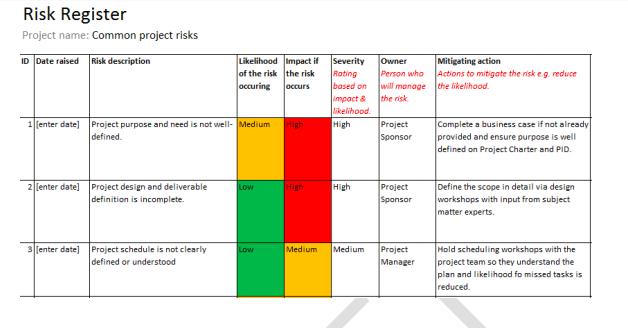
\includegraphics[width=\textwidth]{./Figures/RiskRegisterLNGSTemplate}
\caption{Preliminary Risk Registry Table}
\label{fig:RiskRegistry}
\end{center}
\end{figure}
